%%%%%%%%%%%%%%%%%%%%%%%%%%%%%%%%%%%%%%%%%%%%%%%%%%%%%%%%%%%%%%%%%%%%%
%%                                                                 %%
%% Please do not use \input{...} to include other tex files.       %%
%% Submit your LaTeX manuscript as one .tex document.              %%
%%                                                                 %%
%% All additional figures and files should be attached             %%
%% separately and not embedded in the \TeX\ document itself.       %%
%%                                                                 %%
%%%%%%%%%%%%%%%%%%%%%%%%%%%%%%%%%%%%%%%%%%%%%%%%%%%%%%%%%%%%%%%%%%%%%

%%\documentclass[referee,sn-basic]{sn-jnl}% referee option is meant for double line spacing

%%=======================================================%%
%% to print line numbers in the margin use lineno option %%
%%=======================================================%%

%%\documentclass[lineno,sn-basic]{sn-jnl}% Basic Springer Nature Reference Style/Chemistry Reference Style

%%======================================================%%
%% to compile with pdflatex/xelatex use pdflatex option %%
%%======================================================%%

% \documentclass[pdflatex,sn-mathphys,iicol]{sn-jnl}% Math and Physical Sciences Reference Style
\documentclass[pdflatex,sn-basic,iicol]{sn-jnl}% Math and Physical Sciences Reference Style
\usepackage{lmodern}

\jyear{2021}%

\raggedbottom
%%\unnumbered% uncomment this for unnumbered level heads

\begin{document}

\title[Article]{Furin Cleavage Sites in Sarbecoviruses and Merbecoviruses}

\author[]{\fnm{MouthOfMadness}}

% \affil[]{\orgdiv{Department}, \orgname{Organization}, \orgaddress{\street{Street}, \city{City}, \postcode{100190}, \state{State}, \country{Country}}}

%%==================================%%
%% sample for unstructured abstract %%
%%==================================%%

\abstract{This is a working document for now, to gather ideas and experiments (mostly computationals) around the natural or engineered emergence of Furin Cleavage Sites (FCS) in Sarbecoviruses and Merbecoviruses. We will rely on phylogenetic trees, propabilistic modeling etc.}

%%================================%%
%% Sample for structured abstract %%
%%================================%%

% \abstract{\textbf{Purpose:} The abstract serves both as a general introduction to the topic and as a brief, non-technical summary of the main results and their implications. The abstract must not include subheadings (unless expressly permitted in the journal's Instructions to Authors), equations or citations. As a guide the abstract should not exceed 200 words. Most journals do not set a hard limit however authors are advised to check the author instructions for the journal they are submitting to.
% 
% \textbf{Methods:} The abstract serves both as a general introduction to the topic and as a brief, non-technical summary of the main results and their implications. The abstract must not include subheadings (unless expressly permitted in the journal's Instructions to Authors), equations or citations. As a guide the abstract should not exceed 200 words. Most journals do not set a hard limit however authors are advised to check the author instructions for the journal they are submitting to.
% 
% \textbf{Results:} The abstract serves both as a general introduction to the topic and as a brief, non-technical summary of the main results and their implications. The abstract must not include subheadings (unless expressly permitted in the journal's Instructions to Authors), equations or citations. As a guide the abstract should not exceed 200 words. Most journals do not set a hard limit however authors are advised to check the author instructions for the journal they are submitting to.
% 
% \textbf{Conclusion:} The abstract serves both as a general introduction to the topic and as a brief, non-technical summary of the main results and their implications. The abstract must not include subheadings (unless expressly permitted in the journal's Instructions to Authors), equations or citations. As a guide the abstract should not exceed 200 words. Most journals do not set a hard limit however authors are advised to check the author instructions for the journal they are submitting to.}

\keywords{Sarbecoviruses, Merbecoviruses, FCS}

%%\pacs[JEL Classification]{D8, H51}

%%\pacs[MSC Classification]{35A01, 65L10, 65L12, 65L20, 65L70}

\maketitle

\section{Introduction}\label{intro}
We will try to explore the characteristics in terms of propabilistic models the appearance or presence of furin-like sites. 

We will focus on the following specific polybasic patterns:
\begin{itemize}
    \item $\text{RXXR}$
    \item $\text{RRXR}$ or $\text{RXRR}$
\end{itemize}
These are seen inside the Merbecovirus clade, it was recently demonstrated by \cite{COUTARD2020104742} that an FCS now also exist inside 
the Sarbecovirus clade due to the somewhat unique appearance of the Sars-Cov-2 and all its subsequent variants.

We will also look at quasi-patterns that we will note:
\begin{itemize}
    \item $\overline{\text{RXXR}}$
    \item $\overline{\text{RRXR}}$ or $\overline{\text{RXRR}}$
\end{itemize}
These patterns represent sequences of nucleotides that are one mutation away from their representative pattern.

\subsection{Data and Alignements}
We used two datasets, one for the Merbecoviruses $\Omega_{Merb}$ and one for the Sarbecoviruses $\Omega_{Sarb}$. 
Each dataset was independently aligned using the MAFFT program.
Note that the original Wuhan-Hu-1 is included in $\Omega_{Sarb}$.

\subsection{RNA Stucture}
Following \cite{WU2021102115} we will segment the RNA virus strands in multiple regions. 
As a generic template we can use the structure of the Wuhan-Hu-1 genome (see Fig.\ref{wuhan-hu-1-genome}). 

\begin{figure}[h]
\centering
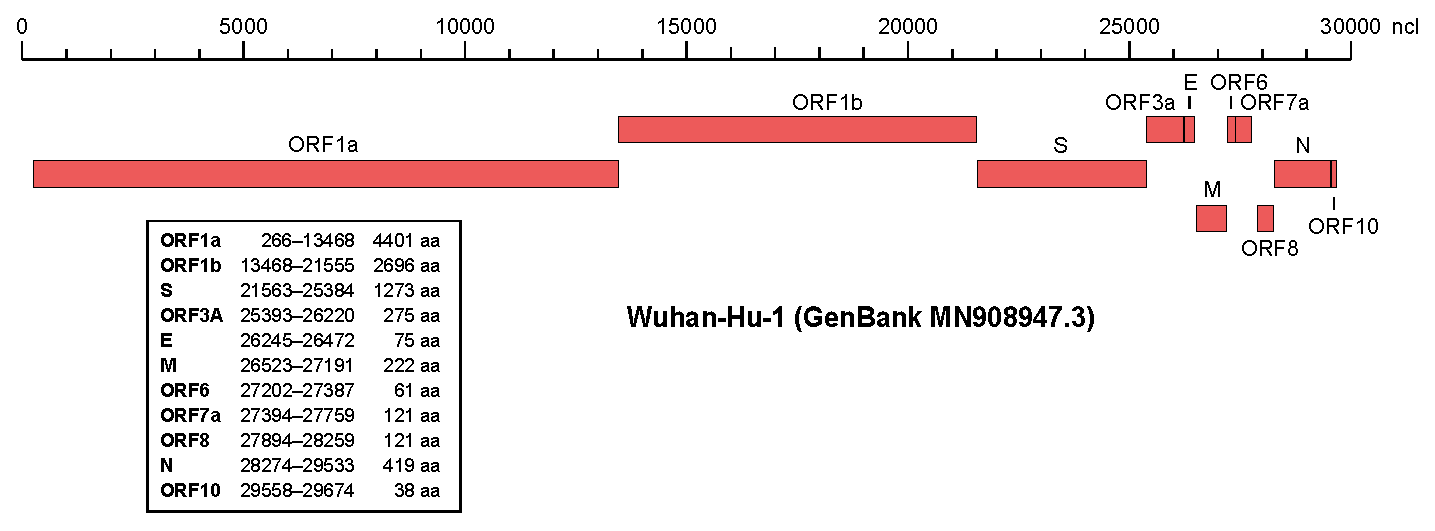
\includegraphics[width=0.45\textwidth]{SARS-CoV-2_genome.eps}
\caption{Wuhan-Hu-1 Genome Structure}\label{wuhan-hu-1-genome}
\end{figure}

Here ORFx are Open Reading Frames that do not encode for structural proteins, 
M (resp. E) stands for the membrane (resp. envelope) protein, N for the nucleocapside (that is responsible for RNA strand packaging), 
and finally $S$ the now infamous spike protein.

We also subdivide the $S$ region in the three following subregions: $S_1$, $S_{link}$ and $S_2$:
\begin{itemize}
    \item $S_1$ represents the first $S$ protein subunit wich contains the Receptor Binding Domain (RBD)
    \item $S_{link}$ the amino-based link between $S_1$ and $S_2$
    \item $S_2$ represents the second $S$ protein subunit.
\end{itemize}

\subsection{Propabilistic Models} 
In the following Sections we will explore different types of propabilistic models. We will start with simple presence models in Sec.\ref{SUM}.

\section{Structural Uniform Model}\label{SUM}
We first focus on a very simple presence model for the FCS patterns. It is based on a piecewise uniform Probability Density Function (pdf).
\[
    f(x) = \left \{  
        \begin{array}{r c l}
            p_{[b]}         & \ & x \in [0, S_1^{b}[        \\
            p_{[S_1]}       & \ & x \in [S_1^{b}, S_1^{e}]  \\
            p_{[S_{link}]}  & \ & x \in ]S_1^{e}, S_2^{b}[  \\
            p_{[S_2]}       & \ & x \in [S_2^{b}, S_2^{e}]   \\
            p_{[e]}         & \ & x \in ]S_2^{e}, N]
        \end{array}   \right . 
\]
We use $b$ (res. $e$) as short mnemonic for $begin$ (resp. $end$). The size of the full RNA strand is $N$.

\subsection{Merbecoviruses $\Omega_{Merb}$}
I will simply report (for now) the results.
\[
    f_{\scriptscriptstyle{\text{RXXR}}}(x) = 1e^{-3} \times \left \{  
        \begin{array}{l l l}
            p_{[b]}         & = 0.525189    & x \in [0, S_1^{b}[        \\
            p_{[S_1]}       & = 0.843278    & x \in [S_1^{b}, S_1^{e}]  \\
            p_{[S_{link}]}  & = 6.61268     & x \in ]S_1^{e}, S_2^{b}[  \\
            p_{[S_2]}       & = 0.491756    & x \in [S_2^{b}, S_2^{e}]   \\
            p_{[e]}         & = 1.02473     & x \in ]S_2^{e}, N]
        \end{array}   \right . 
\]
\[
    f_{\scriptscriptstyle{\overline{\text{RXXR}}}}(x) = 1e^{-2} \times \left \{  
        \begin{array}{l l l}
            p_{[b]}         & = 1.11984     & x \in [0, S_1^{b}[        \\
            p_{[S_1]}       & = 0.757632    & x \in [S_1^{b}, S_1^{e}]  \\
            p_{[S_{link}]}  & = 1.93922     & x \in ]S_1^{e}, S_2^{b}[  \\
            p_{[S_2]}       & = 0.591803    & x \in [S_2^{b}, S_2^{e}]   \\
            p_{[e]}         & = 1.29879     & x \in ]S_2^{e}, N]
        \end{array}   \right . 
\]

\subsection{Sarbecoviruses $\Omega_{Sarb}$}
I will simply report (for now) the results.
\[
    f_{\scriptscriptstyle{\text{RXXR}}}(x) = 1e^{-3} \times \left \{  
        \begin{array}{l l l}
            p_{[b]}         & = 0.327155    & x \in [0, S_1^{b}[        \\
            p_{[S_1]}       & = 0.29627     & x \in [S_1^{b}, S_1^{e}]  \\
            p_{[S_{link}]}  & = 0.0470411   & x \in ]S_1^{e}, S_2^{b}[  \\
            p_{[S_2]}       & = 0.283475    & x \in [S_2^{b}, S_2^{e}]   \\
            p_{[e]}         & = 1.97162     & x \in ]S_2^{e}, N]
        \end{array}   \right . 
\]
\[
    f_{\scriptscriptstyle{\overline{\text{RXXR}}}}(x) = 1e^{-2} \times \left \{  
        \begin{array}{l l l}
            p_{[b]}         & = 1.06255     & x \in [0, S_1^{b}[        \\
            p_{[S_1]}       & = 1.0844      & x \in [S_1^{b}, S_1^{e}]  \\
            p_{[S_{link}]}  & = 0.23991     & x \in ]S_1^{e}, S_2^{b}[  \\
            p_{[S_2]}       & = 1.3954      & x \in [S_2^{b}, S_2^{e}]   \\
            p_{[e]}         & = 1.82017     & x \in ]S_2^{e}, N]
        \end{array}   \right . 
\]


\bibliography{sn-bibliography}% common bib file
%% if required, the content of .bbl file can be included here once bbl is generated
%%\input sn-article.bbl

%% Default %%
%%\input sn-sample-bib.tex%

\end{document}
